% Template for Cogsci submission with R Markdown

% Stuff changed from original Markdown PLOS Template
\documentclass[10pt, letterpaper]{article}

\usepackage{cogsci}
\usepackage{pslatex}
\usepackage{float}
\usepackage{caption}

% amsmath package, useful for mathematical formulas
\usepackage{amsmath}

% amssymb package, useful for mathematical symbols
\usepackage{amssymb}

% hyperref package, useful for hyperlinks
\usepackage{hyperref}

% graphicx package, useful for including eps and pdf graphics
% include graphics with the command \includegraphics
\usepackage{graphicx}

% Sweave(-like)
\usepackage{fancyvrb}
\DefineVerbatimEnvironment{Sinput}{Verbatim}{fontshape=sl}
\DefineVerbatimEnvironment{Soutput}{Verbatim}{}
\DefineVerbatimEnvironment{Scode}{Verbatim}{fontshape=sl}
\newenvironment{Schunk}{}{}
\DefineVerbatimEnvironment{Code}{Verbatim}{}
\DefineVerbatimEnvironment{CodeInput}{Verbatim}{fontshape=sl}
\DefineVerbatimEnvironment{CodeOutput}{Verbatim}{}
\newenvironment{CodeChunk}{}{}

% cite package, to clean up citations in the main text. Do not remove.
\usepackage{apacite}

% KM added 1/4/18 to allow control of blind submission
\cogscifinalcopy

\usepackage{color}

% Use doublespacing - comment out for single spacing
%\usepackage{setspace}
%\doublespacing


% % Text layout
% \topmargin 0.0cm
% \oddsidemargin 0.5cm
% \evensidemargin 0.5cm
% \textwidth 16cm
% \textheight 21cm

\title{Does mere exposure to ideas encourage belief in them?}

\usepackage{booktabs}
\usepackage{longtable}
\usepackage{array}
\usepackage{multirow}
\usepackage{wrapfig}
\usepackage{float}
\usepackage{colortbl}
\usepackage{pdflscape}
\usepackage{tabu}
\usepackage{threeparttable}
\usepackage{threeparttablex}
\usepackage[normalem]{ulem}
\usepackage{makecell}
\usepackage{xcolor}

\author{{\large \bf Justin Mikell (jmikell@asu.edu)} \\ Arizona State University \AND {\large \bf Derek Powell (dmpowell@asu.edu)} \\ School of Social and Behavioral Sciences \\ Arizona State University}

\newlength{\cslhangindent}
\setlength{\cslhangindent}{1.5em}
\newenvironment{CSLReferences}%
  {}%
  {\par}

\begin{document}

\maketitle

\begin{abstract}
Numerous psychological findings have shown that mere exposure to ideas
makes those ideas seem more true, a finding commonly referred to as the
``illusory truth'' effect (e.g. Hasher et al., 1977). In the presence of
pervasive misinformation, this basic feature of cognition may undermine
the functioning of a democratic society (Pennycook et al., 2018).
However, genuine beliefs do not only produce judgments of truth, they
also imply other beliefs and drive decision-making. Here, we sought to
examine whether mere exposure to statements produces genuine beliefs by
examining whether people draw inferences from statements after mere
exposure. Surprisingly, and in contrast to familiarity-based accounts of
the illusory truth effect (e.g. Dechêne et al., 2010), we found that
exposure to ``premise'' statements affected participants' truth ratings
for novel ``implied'' statements. This ``illusory implication'' effect
suggests that exposure to false statements has further-reaching impacts
than previously thought and calls for a new mechanistic account of these
effects.

\textbf{Keywords:}
Illusory truth; Metacognition; Cognitive Psychology; Misinformation
\end{abstract}

Every day, people are faced with a barrage of unsupported claims, from
pestering ad campaigns to blatant disinformation on social media.
Altogether, we live within an information environment that is more
connected and more saturated than ever before in human history
(Bak-Coleman et al., 2021). If we are sufficiently critical consumers of
media, can we benefit from this rich access to information without being
exploited by advertisers or misled by misinformation? Perhaps not.
Numerous psychological findings indicate that mere exposure to ideas
makes those ideas appear more true, a finding commonly referred to as
the ``illusory truth'' effect (De keersmaecker et al., 2020; Dechêne et
al., 2010; Fazio et al., 2015; Hasher et al., 1977; Pennycook et al.,
2018). This effect suggests that we cannot exist in an environment of
mis- and disinformation without being affected by it---without exposure
to these ideas distorting our sense of what is true.

Studies examining the illusory truth effect typically proceed in at
least two phases. At exposure, participants are introduced to a set of
false statements. Typically, the statements are part of a true/false
quiz, or a cover story explains they are part of some other innocuous
judgment task. Then, after some intervening time ranging from minutes to
weeks, participants are asked to judge whether these statements are
true. On average, participants rate the statements as more ``true'' when
they have been exposed to them previously---an illusory truth effect.

Decades of research have demonstrated the consistency and robustness of
the illusory truth effect (e.g.~see Dechêne et al., 2010). The effect
has been demonstrated for frivolous trivia questions (e.g. Hasher et
al., 1977; Lacassagne et al., 2021; Unkelbach, 2007; Wang et al., 2016)
as well as consequential fake news headlines (Pennycook et al., 2018).
The illusory truth effect has also been shown to be robust across people
with different levels of cognitive ability, need for cognitive closure,
and cognitive styles (De keersmaecker et al., 2020).

The effect is one of ``illusory'' truth because it occurs following
``mere exposure'' to statements. That is, it occurs when the statements
are seen or heard in a non-communicative context, such as when they are
read during a true/false quiz. Generally, being told something---even by
a complete stranger of unknown trustworthiness---is prima facie reason
for believing it (Grice, 1989). But reading a statement on a true/false
quiz is not reason for believing it---the statement is being shown only
to test the quiz-taker's knowledge, and is just as likely to be false as
to be true.

There is something unsettling about the illusory truth effect and the
lack of agency it implies over our own beliefs. Even more worrisome,
there could be dire societal implications if merely being exposed to an
idea causes people to adopt it as a belief: Pennycook and colleagues
(2018) argue that the illusory truth effect, combined with an
environment of pervasive misinformation, has important implications for
the functioning of democratic society. The illusory truth effect
suggests that mere exposure to misinformation could have impacts that
cannot be stopped by fact-checking labels (Pennycook et al., 2018), nor
effectively curbed by retractions or corrective information (e.g. Ecker
et al., 2011; Lewandowsky et al., 2012).

However, there is more to \emph{belief} than ratings of truth. To
illustrate, philosophers advancing dispositionalist theories of beliefs
have focused on a number of observable behaviors that are indicative of
belief (Schwitzgebel, 2021). Though a person's assent to a proposition
(whether they agree with or judge it to be truthful) is an important
marker and convenient measure of belief, other features of belief are
just as essential. For instance, beliefs imply other beliefs: for
instance, believing that ``it is sunny out'' implies the belief that
``it is daytime.'' And believing misinformation, such as ``Hillary
Clinton runs a sex-trafficking ring out of a pizza parlor'' (see Robb,
2017) might imply the belief that ``Hillary Clinton would make a bad
president.'' Beliefs also inform action and decision-making, and whether
or not someone holds a belief can be judged (at least partly) from their
decisions. When truly believed, misinformation can have drastic impacts.
To illustrate, a recent study found that people who marked just one
piece of vaccine misinformation as accurate were nearly twice as likely
to be unvaccinated against COVID-19 compared to those who did not
endorse any vaccine misinformation (Ognyanova et al., 2021).

Bearing these features of beliefs in mind, the current state of illusory
truth research does not demonstrate that mere exposure to a statement
truly engenders \emph{belief} in that statement. Consider the mechanisms
thought to underlie the illusory truth effect: most explanations
attribute illusory truth effects to participants' reliance on
familiarity or fluency during the judgment process (Fazio et al., 2015;
Unkelbach, 2007; Wang et al., 2016). Roughly, when asked whether
something is true or false, people search their memory for knowledge
pertaining to belief in the statement, but they also rely on a
meta-cognitive sense of familiarity. Familiarity is a sign that we have
``heard this somewhere before.'' According to foundational theories of
communication, a general assumption that communicators strive to make
true utterances is a prerequisite for successful communication and
social functioning (Grice, 1989). Thus, if having ``heard something
before'' suggests that someone said it, then ecologically this is a
reasonable cue to truth. Psychological studies that elicit the illusory
truth effect hijack this meta-cognitive heuristic: They provide this
sense of familiarity, but from a communicative context that lacks any
reasonable assumption of truth.

This predominant theoretical account suggests that illusory truth
effects do not engender genuine belief and may not have the deleterious
real-world effects that some authors have feared (c.f. Pennycook et al.,
2018). Applying this mechanistic account to the real-world, we might
summarize the most likely process as follows: When people are exposed to
a false statement they form a memory impression of it, but they do not
draw inferences from this statement to revise other beliefs, nor do they
plan future actions on its basis. In a real-world context, there would
be essentially no impact from the exposure. In the experimental context
however, the statement is seen again and a truth-judgment is requested.
It is only at this time that the memory impression of the statement
produces a feeling of familiarity and affects the truth judgments
rendered at that time. Under this theoretical account, the impact of
prior exposure depends on a subsequent re-exposure, coupled with a
judgment or action to be taken at that time. This would make the
real-world consequences of the illusory truth effect far narrower than
some have argued.

Nevertheless, much as we might be relieved to dismiss them, concerns
like those raised by Pennycook and colleagues (2018) loom large enough
to warrant further consideration. Could mere exposure to statements
truly impact beliefs beyond providing a sense of familiarity? Could
illusory truth effects instead reflect genuine belief?

Here, we sought to examine whether the illusory truth effect reflects
genuine beliefs in statements following their mere exposure. One way to
test this is to examine whether people draw inferences from statements
after exposure to those statements in a context without any
presupposition of truth. We designed a study to examine whether mere
exposure to one statement (the ``premise'') could affect truth ratings
for another, different statement that it would logically imply (the
``implication''). Such an ``illusory implication'' effect would
demonstrate that mere-exposure has genuine impacts on beliefs beyond
those explained by familiarity. In contrast, if the illusory truth
effect is caused entirely by feelings of familiarity during the judgment
process, then there should be no effect of prior exposure for new
unfamiliar statements.

\hypertarget{experiment-1}{%
\section{Experiment 1}\label{experiment-1}}

Preregistration information for Experiment 1 can be found at
\url{https://osf.io/c4w8s/}. Materials for both experiments can be found
at \url{https://osf.io/znq3y/}.

\hypertarget{methods}{%
\subsection{Methods}\label{methods}}

\hypertarget{participants}{%
\subsubsection{Participants}\label{participants}}

A total of 400 Participants were recruited through Amazon Mechanical
Turk. Participants who failed basic attention check questions were
excluded from analyses. These questions asked participants to simply
give a particular response. For example, ``This item tests if you are
paying attention, please select `Definitely False.'\,'' At the end of
the study, participants were also asked if they had searched online to
check any of the claims during the experiment (after being reassured
that they would receive compensation regardless of their answers).
Participants who failed any attention checks or who indicated they
searched online were excluded from analysis. This left a final sample of
378 (157 female, median age 36 years-old).

\begin{CodeChunk}
\begin{figure}[h]

{\centering 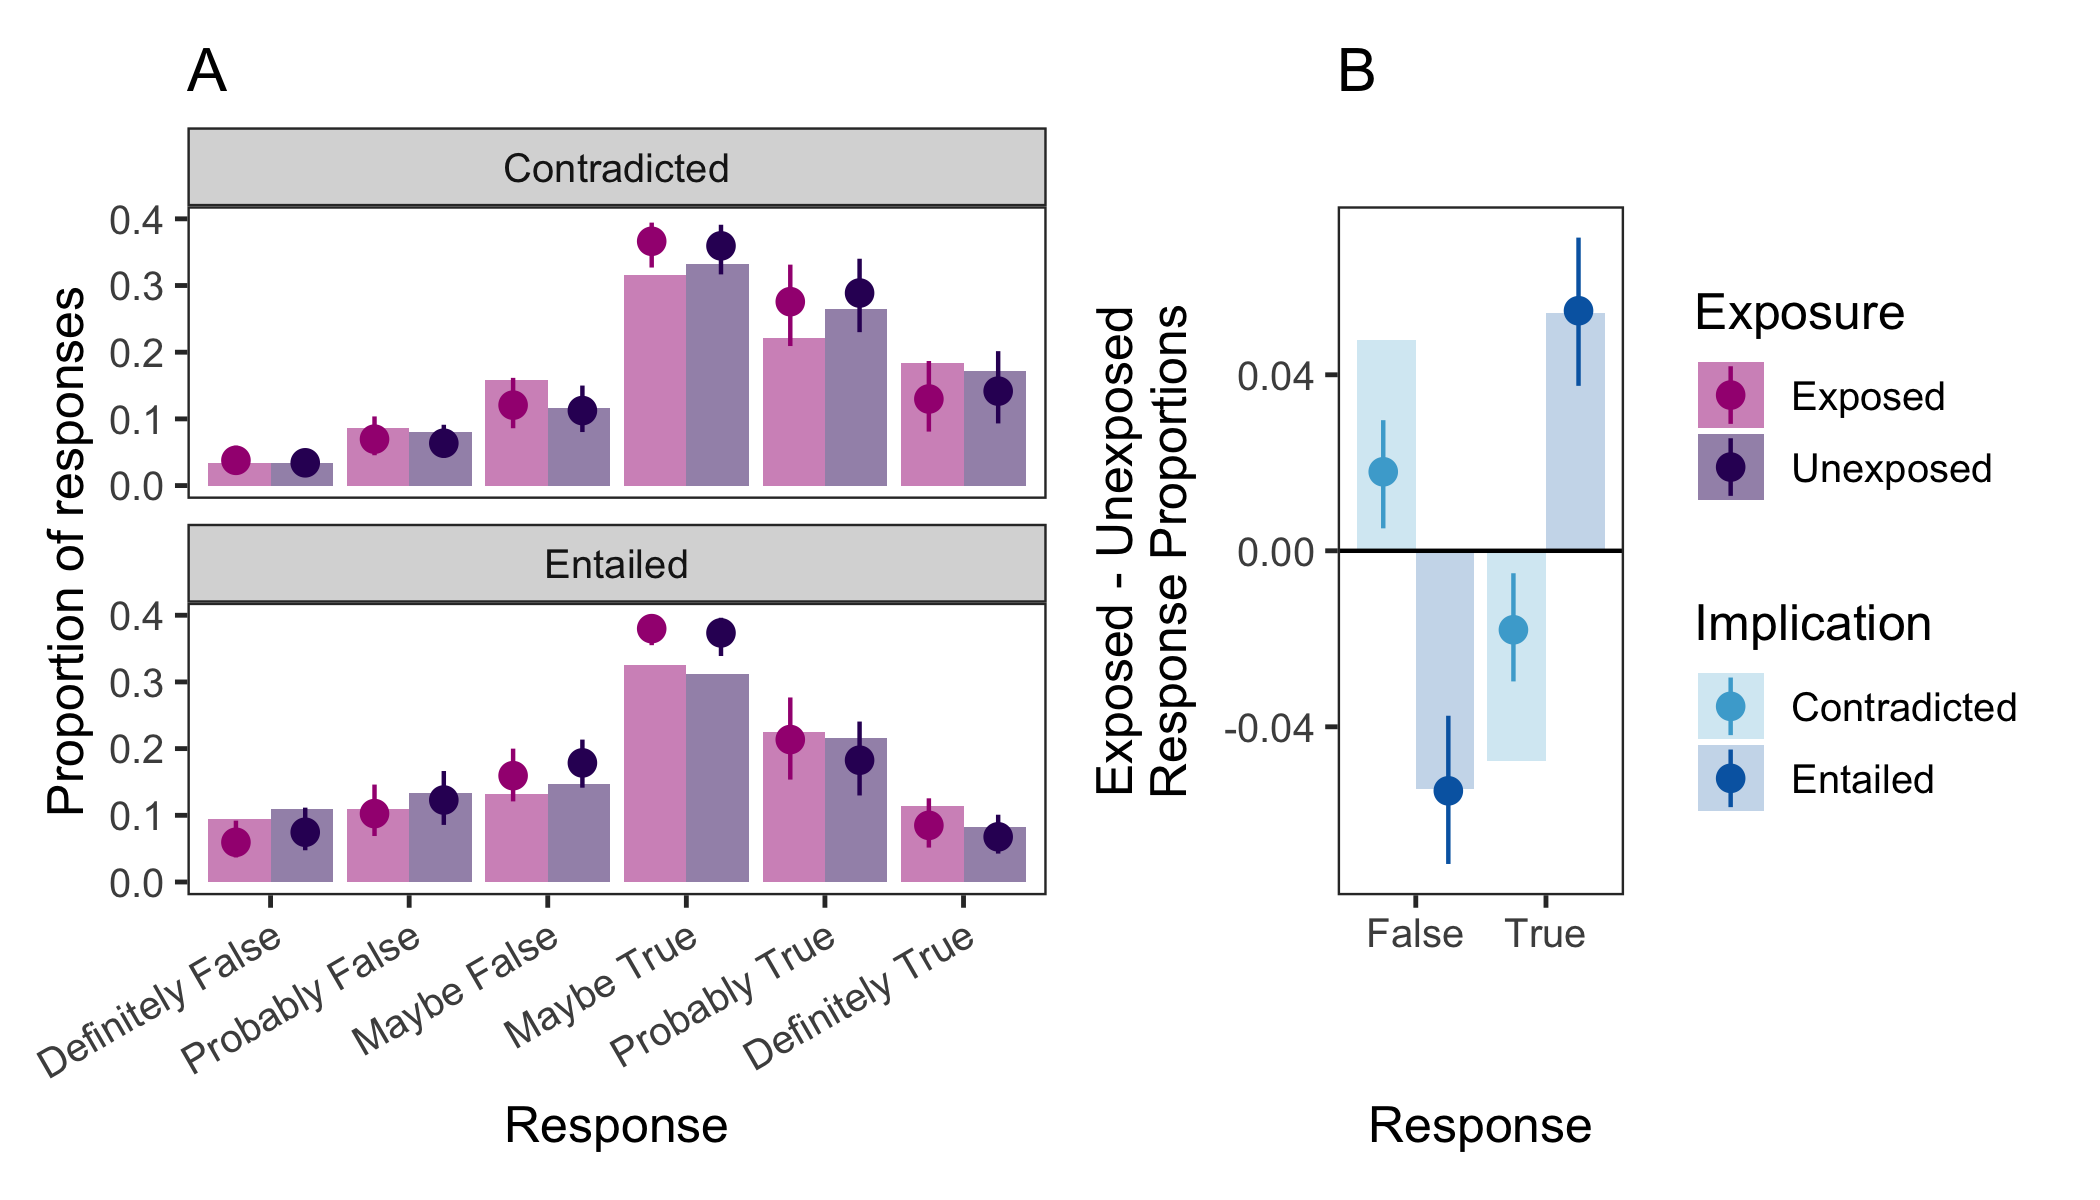
\includegraphics{figs/fig1-1} 

}

\caption[Average truth ratings for Implication statements in Experiment 1, broken down by exposure (exposed vs]{Average truth ratings for Implication statements in Experiment 1, broken down by exposure (exposed vs. unexposed), instructions (fact vs quiz conditions), implication type (true-implied-false vs false-implied-true). For visualization purposes, means were calcaulated by translating ordinal responses onto a scale from -2.5 to 2.5. Error bars indicate standard errors. }\label{fig:fig1}
\end{figure}
\end{CodeChunk}

\hypertarget{materials}{%
\subsubsection{Materials}\label{materials}}

We created 24 pairs of statements presenting claims about history. Each
pair consisted of a ``premise'' statement and a ``implied'' statement.
Each ``premise'' statement was a falsehood that implied either the truth
or falsity of the ``implied'' statement. Of the pairs, 12 had premise
statements implying that a true statement was false (true-implied-false)
and the other 12 had premise statements implying another false statement
was true (false-implied-true). For instance, one ``true-implied-false''
pair was the premise statement, ``No U.S. astronauts have died since the
Challenger explosion in 1986'' paired with the implied statement, ``The
space shuttle Columbia disintegrated over Texas in 2003'' (true, but
implied to be false by the ``premise''). An example of a
``false-implied-true'' pair was the premise statement, ``The Tour de
France has been held every year since its inception in 1903'' paired
with the implied statement, ``The Tour de France was still held during
WWI and WWII'' (false, but implied true by the ``premise'').

\hypertarget{procedures}{%
\subsubsection{Procedures}\label{procedures}}

Participants first completed informed consent and a Captcha to limit bot
participation.

The study proceeded in three phases: 1) an exposure phase, 2) a
distraction phase, 3) and finally a testing phase. At the exposure
phase, participants were presented with a subset of the ``premise''
statements (8 of the 24 total) as well as some control statements (12
true, 4 false). Then, after the distraction phase, the testing phase
consisted of a true-or-false quiz. The items tested included both
``premise'' and ``implied'' statements from the 24 item-pairs. For some
of the tested ``implied'' statements, participants had previously seen
the related ``premise'' statement (exposed implied test). For others,
they had not seen the related statements (unexposed implied test).
Similarly, they were tested on the ``premise'' statements they had
previously seen during the exposure phase (exposed premise test) as well
as new unseen premise statements (for which they had also not seen the
related implied statements). Participants were randomly assigned into
three counterbalancing conditions that varied which of the
statement-pairs were assigned to each exposure/test combination.

At the beginning of the study, participants were randomly assigned to
either the ``fact'' (\emph{n} = 100) or ``quiz'' (\emph{n} = 300)
exposure condition and to one of three counterbalancing conditions.
Participants assigned to the quiz and fact conditions received different
instructions and performed different tasks in the exposure phase.

Participants in the fact condition were told the study's main purpose
was to learn more about how people learn and apply new knowledge. They
were informed that the initial set of statements they would see were all
facts, and were asked to rate how surprising each ``fact'' was to them.
The true purpose of this condition was to test whether participants
would successfully draw inferences from the ``premise'' to the
``implied'' statements when told that the premises were true.

Participants in the quiz condition were told that they were to be given
a true/false quiz, so that some of the statements would be true and some
false. These participants rated how confident they were that each of the
presented statements were true or false. The purpose of the quiz
condition was to provide ``mere exposure'' to these statements, to test
for illusory truth and illusory implication effects. We tested for the
illusory truth effect by comparing truth ratings for premise statements
seen during exposure to those that had not been seen. Similarly, we
tested for the illusory implication effect by comparing truth ratings
for implication statements whose corresponding premise statements were
and were not presented during the exposure phase. If mere exposure to
``premise'' statements affects participants' judgments of the
``implied'' statements, this would be evidence for an illusory
implication effect.

After their initial exposure to the statements, participants provided
basic demographic information and were then presented with the expanded
7 question version of the Cognitive Reflection Task (CRT, Frederick,
2005; Toplak et al., 2014). These tasks served to provide a period of
distraction between exposure and test.

Then, participants advanced to the testing phase, where all participants
were asked to rate their confidence that each statement was true or
false. These ratings were made on a 6-point scale from ``Definitely
False'' to ``Definitely True.'' The test phase consisted of the 8
premise statements the participants previously saw, their respective
matching 8 implication statements, 8 novel implication statements, 8
previously unseen premise statements, 12 true control statements, and 4
false control statements.

At the end of the study, participants were debriefed and presented with
a list of the false statements they had seen.

\hypertarget{results-and-discussion}{%
\subsection{Results and discussion}\label{results-and-discussion}}

Participants made their truth ratings in the test phase on a 6-point
scale from ``Definitely false'' to ``Definitely true.'' To properly
treat these Likert-style responses, the truth ratings were analyzed
using multilevel Bayesian cumulative ordinal regression models (Bürkner
\& Vuorre, 2019) with random intercepts and slopes for participants and
items. Cumulative ordinal regression models assume that participants'
discrete responses are driven by a continuous latent variable and a set
of k-1 thresholds determining the range of the continuous variable
corresponding to each of the ordinal response options. This model helps
to account for potential differences in scale usage as well as the
bounded nature of the response scale.

All models were fit using the brms R package (Bürkner, 2017), with model
posteriors estimated using the No-U-Turn Markov Chain Monte Carlo (MCMC)
sampler implemented in Stan. Four MCMC chains were run for each model,
with 2000 samples (1000 burn-in) drawn from each. Chains were assessed
for convergence with \(\hat{R}\) and the total estimated effective
sample size was verified to be greater than 1000 for all parameters
(Gelman et al., 2014).

\hypertarget{fact-condition}{%
\subsubsection{Fact condition}\label{fact-condition}}

First, we examined truth ratings for the premise and implications
statements among participants who were told that the false statements
were true at exposure (``fact'' condition). As expected, exposure to the
premise statements when presented as ``facts'' increased endorsement at
test, \(\beta =\) 1.193, 95\% CI {[}0.987, 1.388{]}. In addition,
participants successfully drew inferences from these ``facts,''
resulting in decreased accuracy for the implication statements at test,
\(\beta =\) -0.345, 95\% CI {[}-0.601, -0.098{]}.

\hypertarget{quiz-condition}{%
\subsubsection{Quiz condition}\label{quiz-condition}}

It is quite appropriate that people should draw new inferences when they
learn new facts. But would participants' endorsements of the implication
statements be affected by mere exposure to the premise statements in the
``quiz'' condition? To our surprise, it appears that they were. Figure 1
shows participants' average truth ratings for the implication statements
in the quiz condition. Participants gave higher truth ratings following
exposure for false statements implied to be true, and somewhat lower
truth ratings following exposure for true statements implied to be
false.

\begin{CodeChunk}
\begin{table}

\caption{\label{tab:make-tables}Population coefficients of Bayesian regression model for Implication effects in Experiment 1.}
\centering
\begin{tabular}[t]{lrrr}
\toprule
Term & Estimate & $CI_{2.5\%}$ & $CI_{97.5\%}$\\
\midrule
Intercept[1] & -3.38 & -3.86 & -2.92\\
Intercept[2] & -2.26 & -2.74 & -1.80\\
Intercept[3] & -1.36 & -1.83 & -0.91\\
Intercept[4] & 0.27 & -0.20 & 0.72\\
Intercept[5] & 1.80 & 1.34 & 2.27\\
\addlinespace
familiarity & 0.07 & -0.09 & 0.23\\
implication & 0.17 & 0.00 & 0.35\\
implication type & -0.84 & -1.47 & -0.19\\
\bottomrule
\end{tabular}
\end{table}

\end{CodeChunk}

\begin{CodeChunk}
\begin{table}

\caption{\label{tab:make-tables}Population coefficients of Bayesian regression model for Implication effects in Experiment 2.}
\centering
\begin{tabular}[t]{lrrr}
\toprule
Term & Estimate & $CI_{2.5\%}$ & $CI_{97.5\%}$\\
\midrule
Intercept[1] & -3.17 & -3.58 & -2.73\\
Intercept[2] & -2.04 & -2.44 & -1.61\\
Intercept[3] & -1.18 & -1.58 & -0.75\\
Intercept[4] & 0.36 & -0.03 & 0.80\\
Intercept[5] & 1.93 & 1.52 & 2.36\\
\addlinespace
familiarity & 0.13 & -0.03 & 0.29\\
implication & 0.38 & 0.21 & 0.55\\
implication type & -0.79 & -1.36 & -0.21\\
\bottomrule
\end{tabular}
\end{table}

\end{CodeChunk}

An increase in truth ratings for the false-implied-true statements could
potentially be explained by familiarity. This would be consistent with
findings from Arkes and colleagues (1991), who found evidence for
illusory truth for novel statements that were on the same topic as
previously-seen statements. However, familiarity cannot explain the
decrease in truth ratings for the true-implied-false items, as
familiarity should encourage uniformly higher, not lower, truth ratings.

A regression model was used to tease apart the effects of familiarity
and logical implication. The model includes a) a binary variable
indicating the type of implication statement (true-implied-false or
false-implied-true), b) a binary predictor for prior exposure to the
related premise coded zero when the premise was not seen and 1 when it
was seen (capturing potential effects of familiarity), c) and a variable
capturing the effect of implications, coded 1 for implied truth, -1 for
implied falsehood, and zero when the related premise statement was not
seen at exposure. Thus the ``implication'' predictor accounts for the
effect of exposure to the premise on truth judgments for the implied
statements (either positive or negative), while the ``familiarity''
predictor accounts for any positive effect of familiarity. We also
incorporated ``maximal'' random intercepts and slopes for all terms
varying by subject and item (Barr et al., 2013). Expressed in the common
``lme4'' syntax (Bates et al., 2015), the regression model:

\begin{align*}
\text{response} \sim 
 \text{item type} &+ \text{familiarity} + \text{implication} \\
&+ (1 + \text{familiarity} + \text{implication}|\text{subject}) \\
&+ (1 + \text{familiarity} + \text{implication}|\text{item})
\end{align*}

Table 1 presents a summary of the posterior distribution estimated for
the population-level coefficients in this model. The results indicate
that both familiarity and the implication of the premise statements
affected participants' truth ratings. The implication effect is very
credibly greater than zero. To judge its overall magnitude, we compared
the parameter estimate to the parameter estimate from the same
regression model applied to participants' responses in the ``fact''
condition (\(\beta =\) 0.532, 95\% CI {[}0.215, 0.848{]}). Although
smaller than the effect observed in the ``fact'' condition, the effect
in the ``quiz'' condition is of a similar order of magnitude.

Surprisingly, the effects of exposure on participants' truth ratings for
the premise statements were very subtle. Our primary preregistered test
compared participants' truth ratings for the exposed premise statements
at test against their ratings for another set of 8 unexposed premise
statements. This analysis did not find any evidence of an illusory truth
effect, with a posterior estimate for the exposure parameter that
credibly included zero. However, a secondary preregistered analysis
comparing participants' initial truth judgments for the
premise-statements to their later truth judgments for those same
statements at test did find a credible increase in endorsements,
\(\beta =\) 0.213, 95\% CI {[}0.078, 0.345{]}.

The small size of these illusory truth effects may owe to the use of a
``quiz'' judgment task at exposure as well as the relatively brief
period of distraction between exposure and test used in Experiment 1. By
first responding to the statements in a quiz, participants may then have
felt pressure to maintain consistency in their responses, and may have
still possessed some explicit memory of their responses for the premise
statements. If so, this could have suppressed the influence of
familiarity traditionally argued to produce the illusory truth effect.

More importantly, a drive to maintain consistency might also explain our
surprising findings of an illusory implication effect. Participants
showed a general bias toward judging statements ``true'' during the
exposure phase, responding with some variation of ``true'' for 71.8\% of
responses. Attempting to maintain consistency with these prior responses
could have thus influenced their responses to the implication
statements, rendering the observed effect an artifact of the
experimental context.

\hypertarget{experiment-2}{%
\section{Experiment 2}\label{experiment-2}}

Experiment 2 was conducted to address the possibility that a pressure
for internal consistency produced the effects on the
implication-statement truth ratings observed in Experiment 1.
Preregistration informationExperiment 2 can be found at
\url{https://osf.io/czkdh/}.

\begin{CodeChunk}
\begin{figure}[t]

{\centering 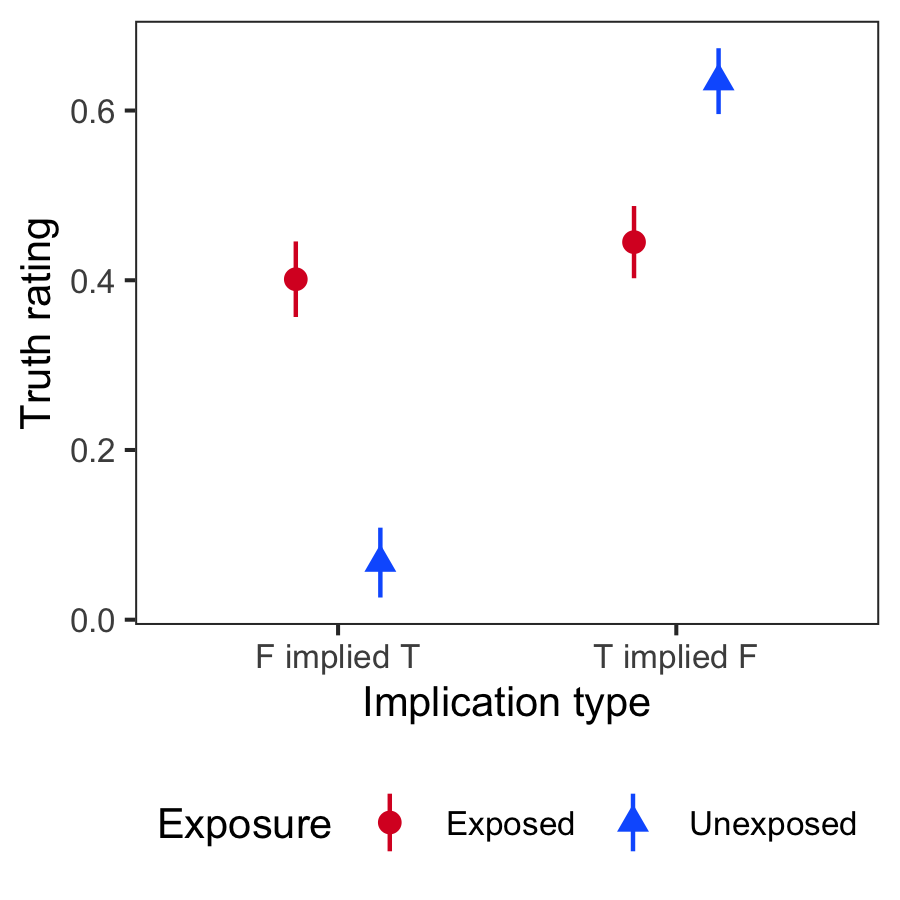
\includegraphics{figs/fig2-1} 

}

\caption[Average truth ratings for Implication statements in Experiment 2, broken down by exposure (exposed vs]{Average truth ratings for Implication statements in Experiment 2, broken down by exposure (exposed vs. unexposed) and implication type (true-implied-false vs false-implied-true). For visualization purposes, means were calcaulated by translating ordinal responses onto a scale from -2.5 to 2.5. Error bars indicate standard errors.}\label{fig:fig2}
\end{figure}
\end{CodeChunk}

\hypertarget{methods-1}{%
\subsection{Methods}\label{methods-1}}

\hypertarget{participants-1}{%
\subsubsection{Participants}\label{participants-1}}

A total of 300 participants were recruited from Amazon Mechanical Turk
using procedures identical to Experiment 1. As before, participants who
failed attention check questions or who indicated they had looked up
answers were excluded from analyses, leaving a final sample of 286 (157
female, median age 38 years-old).

\hypertarget{materials-and-procedures}{%
\subsubsection{Materials and
procedures}\label{materials-and-procedures}}

All items and procedures were identical to Experiment 1 except for three
changes.

First, all participants were assigned to a new ``interest'' condition.
At exposure, participants were told that they would see a set of
statements, some true and some false, and they were instructed to rate
how interesting each statement was. This change was made to avoid
forcing participants to make a true/false judgment for the exposed
premise-statements, which could have pushed them to try to make coherent
or consistent responses to the related implication-statements.
Importantly, as with a true/false quiz, the presentation of statements
in this context should not warrant any inference as to the truth of
those statements.

Secondly, to provide a longer period of distraction between exposure and
test, the ordering of the items in the test phase was rearranged.
Participants first rated 24 control items (12 true and 12 false) to
extend the time between rating main test items.

Third, another change in test presentation order further prevented any
consistency-pressure: Participants judged the truth of all of the
implication statements before judging the premise statements.

\hypertarget{results-and-discussion-1}{%
\subsection{Results and discussion}\label{results-and-discussion-1}}

Figure 2 shows participants' average truth ratings for the implication
statements with and without exposure to their corresponding premise
statements in Experiment 2. The illusory implication effect was again
observed. As shown in the figure, truth ratings were clearly affected by
exposure: participants gave higher truth ratings following exposure for
false statements implied to be true, and lower truth ratings following
exposure for true statements implied to be false. Table 2 shows the
posterior population-level estimates for an identical regression as was
conducted for Experiment 1. Experiment 2 replicated the effects of
Experiment 1 in a revised design that eliminated any consistency
pressure or demands on participants. In fact, the magnitude of the
effect for the implication statements was somewhat larger in Experiment
2 than in Experiment 1.

\begin{CodeChunk}
\begin{figure*}[!hbt]

{\centering 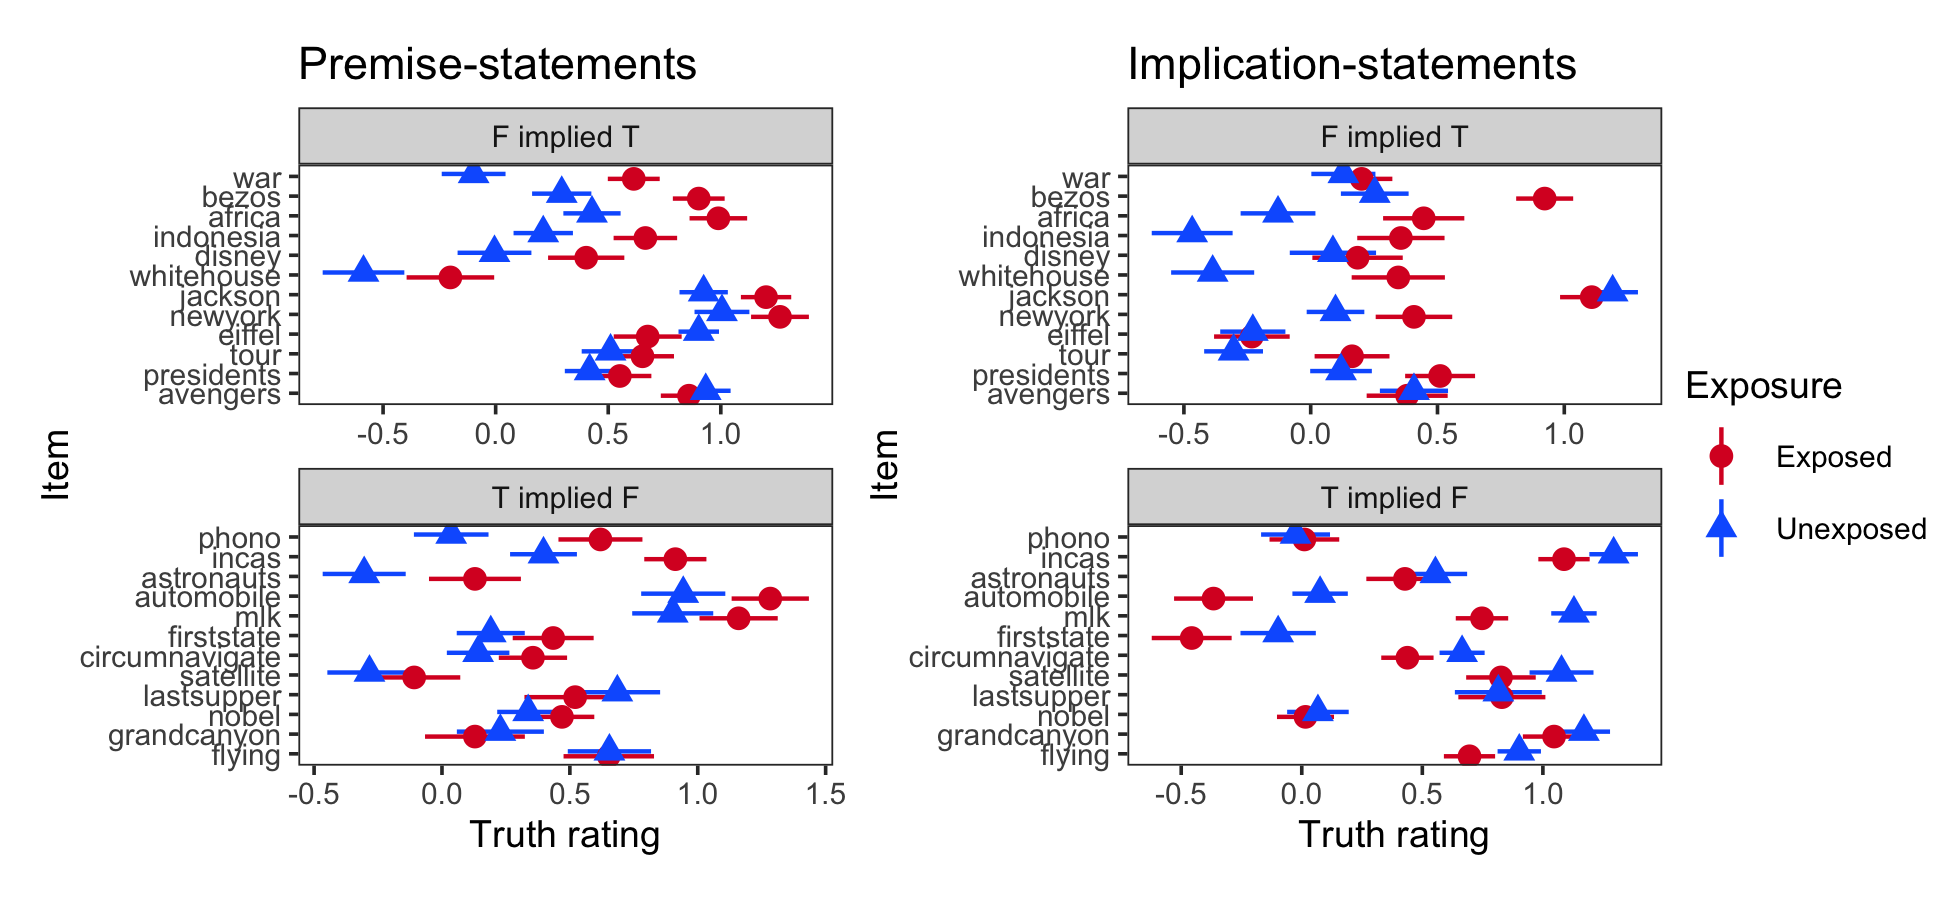
\includegraphics{figs/fig3-1} 

}

\caption[Average truth ratings for individual premise and implication statements in Experiment 2, broken down by exposure (exposed vs]{Average truth ratings for individual premise and implication statements in Experiment 2, broken down by exposure (exposed vs. unexposed) and implication type (true-implied-false vs false-implied-true). For visualization purposes, means were calcaulated by translating ordinal responses onto a scale from -2.5 to 2.5. Error bars indicate standard errors.}\label{fig:fig3}
\end{figure*}
\end{CodeChunk}

In addition, participant's truth ratings for the premise statements in
Experiment 2 revealed the classic illusory truth effect: premise
statements were rated as more true when participants had been exposed to
them previously \(\beta =\) 0.525, 95\% CI {[}0.333, 0.719{]}.

Interestingly, though somewhat smaller, the illusory implication effect
for the implication statements was generally similar in magnitude to the
illusory truth effect observed among the premise statements.

One limitation of these studies relative to prior work on the illusory
truth effect is the relatively limited number of statements participants
saw and were tested on. Generating diverse pairs of statements with a
clear implication relation is relatively more challenging than simply
generating false statements. Fortunately as shown in Figure 3, the
illusory implication effect was fairly robust across the majority of the
24 different individual item pairs in Experiment 2.

\hypertarget{discussion}{%
\section{Discussion}\label{discussion}}

We observed an ``illusory implication'' effect across two preregistered
experiments: mere exposure to premises (e.g.~that ``The Tour de France
has been held every year since its inception in 1903'') influenced
participant's truth ratings for examples of their logical implications
(e.g.~that ``The Tour de France was still held during World War I and
World War II''). Unlike the illusory truth effect, this novel effect
cannot be easily explained by the effects of familiarity or fluency on
the judgment process (cf. Fazio et al., 2015; Unkelbach, 2007; Wang et
al., 2016): whereas familiarity would be expected to uniformly increase
endorsements, participants' truth ratings for implication statements
were both increased and decreased according to the implications of the
corresponding premises. Thus, it appears that mere exposure has a
genuine impression on people's beliefs beyond simply creating a sense of
familiarity.

If not familiarity, then what cognitive mechanism could explain these
findings? One potential explanation is that mere exposure to the premise
statements essentially leads participants to at least partially adopt
the premise statements as beliefs. Simply entertaining the idea may
create such an impression despite awareness of its ambiguous
truth-value. Or, consistent with a general overriding expectation of
truth in testimony (e.g. Grice, 1989; Levine, 2014), participants may at
least partially accept the premise statements as true despite the
experimental context making clear they should not. This explanation
would be consistent with the general truth-bias observed throughout both
studies. Future research might vary the plausibility of the premise
statements to evaluate this explanation or identify its boundary
conditions (Fazio et al., 2019).

Another potential explanation would attribute the illusory implication
effect to processes that play out in the testing phase. Rather than
familiarity, the illusory implication effect may instead reflect
explicit memory and source misattribution: Participants may (at least
partially) remember the premise statements, but fail to properly
attribute their source to the experimental context. Future research
might explore how explicit memory for the premise statements correlates
with the strength of the illusory implication effects. In particular,
research might disentangle memory effects by exploring factors that are
known to affect memory, but that should not affect other reasoning
processes, such as retention intervals or serial-position effects (e.g.
Bjork \& Whitten, 1974).

Finally, given the surprising nature of our findings, we must raise the
possibility of potential deflationary explanations: that the finding
could be some kind of experimental demand characteristic. For instance,
participants' might imagine there is some kind of trick so that they are
expected to reason forward from the initial exposure to the items. Or,
some proportion might have been sufficiently confused so as to imagine
they were meant to believe the statements on their initial exposure
(though it is hard to imagine this in Experiment 1). Further work should
explore participants' perceptions of the purposes of these studies and
the potential for different response strategies. However, it should be
noted that similar concerns could be levied at essentially all prior
research on the illusory truth effect.

Whatever the cognitive mechanism behind the illusory implication effect
we observed, these findings are further cause for concern about the
spread of misinformation on and offline. The spread of misinformation
and fake news may outpace the spread of factual news (Vosoughi et al.,
2018) and creates massive challenges for online platforms seeking to
remove, label, and correct misinformation (Sharma et al., 2019). These
challenges may be further compounded by basic features of human
cognition: mere exposure to false statements can make them appear true.
Further, as our findings are the first to indicate, these impacts
generalize to related statements and are potentially indicative of
genuine belief following mere exposure.

\hypertarget{references}{%
\section{References}\label{references}}

\setlength{\parindent}{-0.1in} 
\setlength{\leftskip}{0.125in}

\noindent

\hypertarget{refs}{}
\begin{CSLReferences}
\leavevmode\hypertarget{ref-arkes.etal1991}{}%
Arkes, H. R., Boehm, L. E., \& Xu, G. (1991). Determinants of judged
validity. \emph{Journal of Experimental Social Psychology},
\emph{27}(6), 576--605.
\url{https://doi.org/10.1016/0022-1031(91)90026-3}

\leavevmode\hypertarget{ref-bak-coleman.etal2021}{}%
Bak-Coleman, J. B., Alfano, M., Barfuss, W., Bergstrom, C. T., Centeno,
M. A., Couzin, I. D., Donges, J. F., Galesic, M., Gersick, A. S.,
Jacquet, J., Kao, A. B., Moran, R. E., Romanczuk, P., Rubenstein, D. I.,
Tombak, K. J., Bavel, J. J. V., \& Weber, E. U. (2021). Stewardship of
global collective behavior. \emph{Proceedings of the National Academy of
Sciences}, \emph{118}(27). \url{https://doi.org/10.1073/pnas.2025764118}

\leavevmode\hypertarget{ref-barr.etal2013}{}%
Barr, D. J., Levy, R., Scheepers, C., \& Tily, H. J. (2013). Random
effects structure for confirmatory hypothesis testing: {Keep} it
maximal. \emph{Journal of Memory and Language}, \emph{68}(3),
10.1016/j.jml.2012.11.001.
\url{https://doi.org/10.1016/j.jml.2012.11.001}

\leavevmode\hypertarget{ref-bates.etal2015}{}%
Bates, D., Mächler, M., Bolker, B., \& Walker, S. (2015). Fitting
{Linear} {Mixed}-{Effects} {Models} {Using} \textbf{lme4}. \emph{Journal
of Statistical Software}, \emph{67}(1).
\url{https://doi.org/10.18637/jss.v067.i01}

\leavevmode\hypertarget{ref-bjork.whitten1974}{}%
Bjork, R. A., \& Whitten, W. B. (1974). Recency-sensitive retrieval
processes in long-term free recall. \emph{Cognitive Psychology},
\emph{6}(2), 173--189.
\url{https://doi.org/10.1016/0010-0285(74)90009-7}

\leavevmode\hypertarget{ref-burkner2017}{}%
Bürkner, P.-C. (2017). \textbf{Brms} : {An} \emph{r} {Package} for
{Bayesian} {Multilevel} {Models} {Using} \emph{stan}. \emph{Journal of
Statistical Software}, \emph{80}(1).
\url{https://doi.org/10.18637/jss.v080.i01}

\leavevmode\hypertarget{ref-burkner.vuorre2019}{}%
Bürkner, P.-C., \& Vuorre, M. (2019). Ordinal {Regression} {Models} in
{Psychology}: {A} {Tutorial}. \emph{Advances in Methods and Practices in
Psychological Science}, \emph{2}(1), 77--101.
\url{https://doi.org/10.1177/2515245918823199}

\leavevmode\hypertarget{ref-dekeersmaecker.etal2020}{}%
De keersmaecker, J., Dunning, D., Pennycook, G., Rand, D. G., Sanchez,
C., Unkelbach, C., \& Roets, A. (2020). Investigating the {Robustness}
of the {Illusory} {Truth} {Effect} {Across} {Individual} {Differences}
in {Cognitive} {Ability}, {Need} for {Cognitive} {Closure}, and
{Cognitive} {Style}. \emph{Personality and Social Psychology Bulletin},
\emph{46}(2), 204--215. \url{https://doi.org/10.1177/0146167219853844}

\leavevmode\hypertarget{ref-dechene.etal2010}{}%
Dechêne, A., Stahl, C., Hansen, J., \& Wänke, M. (2010). The {Truth}
{About} the {Truth}: {A} {Meta}-{Analytic} {Review} of the {Truth}
{Effect}. \emph{Personality and Social Psychology Review}, \emph{14}(2),
238--257. \url{https://doi.org/10.1177/1088868309352251}

\leavevmode\hypertarget{ref-ecker.etal2011}{}%
Ecker, U. K. H., Lewandowsky, S., Swire, B., \& Chang, D. (2011).
Correcting false information in memory: {Manipulating} the strength of
misinformation encoding and its retraction. \emph{Psychonomic Bulletin
\& Review}, \emph{18}(3), 570--578.
\url{https://doi.org/10.3758/s13423-011-0065-1}

\leavevmode\hypertarget{ref-fazio.etal2015}{}%
Fazio, L. K., Brashier, N. M., Payne, B. K., \& Marsh, E. J. (2015).
Knowledge does not protect against illusory truth. \emph{Journal of
Experimental Psychology: General}, \emph{144}(5), 993--1002.
\url{https://doi.org/10.1037/xge0000098}

\leavevmode\hypertarget{ref-fazio.etal2019}{}%
Fazio, L. K., Rand, D. G., \& Pennycook, G. (2019). Repetition increases
perceived truth equally for plausible and implausible statements.
\emph{Psychonomic Bulletin \& Review}, \emph{26}(5), 1705--1710.
\url{https://doi.org/10.3758/s13423-019-01651-4}

\leavevmode\hypertarget{ref-frederick2005}{}%
Frederick, S. (2005). Cognitive {Reflection} and {Decision} {Making}.
\emph{Journal of Economic Perspectives}, \emph{19}(4), 25--42.
\url{https://doi.org/10.1257/089533005775196732}

\leavevmode\hypertarget{ref-gelman.etal2014}{}%
Gelman, A., Carlin, J. B., Stern, H. S., Dunson, D. B., Vehtari, A., \&
Rubin, D. B. (2014). \emph{Bayesian data analysis} (Third edition). CRC
Press.

\leavevmode\hypertarget{ref-grice1989}{}%
Grice, H. P. (1989). \emph{Studies in the way of words}. Harvard
university press.

\leavevmode\hypertarget{ref-hasher.etal1977}{}%
Hasher, L., Goldstein, D., \& Toppino, T. (1977). Frequency and the
conference of referential validity. \emph{Journal of Verbal Learning and
Verbal Behavior}, \emph{16}(1), 107--112.
\url{https://doi.org/10.1016/S0022-5371(77)80012-1}

\leavevmode\hypertarget{ref-lacassagne.etal2021}{}%
Lacassagne, D., Béna, J., \& Corneille, O. (2021). \emph{Is {Earth} a
{Perfect} {Square}? {Repetition} {Increases} the {Perceived} {Truth} of
{Highly} {Implausible} {Statements}}. PsyArXiv.
\url{https://doi.org/10.31234/osf.io/fce8z}

\leavevmode\hypertarget{ref-levine2014}{}%
Levine, T. R. (2014). Truth-{Default} {Theory} ({TDT}): {A} {Theory} of
{Human} {Deception} and {Deception} {Detection}. \emph{Journal of
Language and Social Psychology}, \emph{33}(4), 378--392.
\url{https://doi.org/10.1177/0261927X14535916}

\leavevmode\hypertarget{ref-lewandowsky.etal2012}{}%
Lewandowsky, S., Ecker, U. K. H., Seifert, C. M., Schwarz, N., \& Cook,
J. (2012). Misinformation and {Its} {Correction}: {Continued}
{Influence} and {Successful} {Debiasing}. \emph{Psychological Science in
the Public Interest}, \emph{13}(3), 106--131.
\url{https://doi.org/10.1177/1529100612451018}

\leavevmode\hypertarget{ref-ognyanova.etal2021}{}%
Ognyanova, K., Lazer, D., Baum, M., Druckman, J., Green, J., Perlis, R.
H., Santillana, M., Simonson, M. D., Lin, J., \& Uslu, A. (2021).
\emph{The {COVID} {States} {Project} \#60: {COVID}-19 vaccine
misinformation: {From} uncertainty to resistance}. OSF Preprints.
\url{https://doi.org/10.31219/osf.io/xtjad}

\leavevmode\hypertarget{ref-pennycook.etal2018}{}%
Pennycook, G., Cannon, T. D., \& Rand, D. G. (2018). Prior exposure
increases perceived accuracy of fake news. \emph{Journal of Experimental
Psychology: General}, \emph{147}(12), 1865--1880.
https://doi.org/\url{http://dx.doi.org/10.1037/xge0000465}

\leavevmode\hypertarget{ref-robb2017}{}%
Robb, A. (2017). Pizzagate: {Anatomy} of a {Fake} {News} {Scandal}. In
\emph{Rolling Stone}.
\url{https://www.rollingstone.com/feature/anatomy-of-a-fake-news-scandal-125877/}

\leavevmode\hypertarget{ref-schwitzgebel2021}{}%
Schwitzgebel, E. (2021). Belief. In E. N. Zalta (Ed.), \emph{The
{Stanford} {Encyclopedia} of {Philosophy}} (Winter 2021). Metaphysics
Research Lab, Stanford University.
\url{https://plato.stanford.edu/archives/win2021/entries/belief/}

\leavevmode\hypertarget{ref-sharma.etal2019}{}%
Sharma, K., Qian, F., Jiang, H., Ruchansky, N., Zhang, M., \& Liu, Y.
(2019). Combating {Fake} {News}: {A} {Survey} on {Identification} and
{Mitigation} {Techniques}. \emph{ACM Transactions on Intelligent Systems
and Technology}, \emph{10}(3), 1--42.
\url{https://doi.org/10.1145/3305260}

\leavevmode\hypertarget{ref-toplak.etal2014}{}%
Toplak, M. E., West, R. F., \& Stanovich, K. E. (2014). Assessing
miserly information processing: {An} expansion of the {Cognitive}
{Reflection} {Test}. \emph{Thinking \& Reasoning}, \emph{20}(2),
147--168. \url{https://doi.org/10.1080/13546783.2013.844729}

\leavevmode\hypertarget{ref-unkelbach2007}{}%
Unkelbach, C. (2007). Reversing the {Truth} {Effect}: {Learning} the
{Interpretation} of {Processing} {Fluency} in {Judgments} of {Truth}.
\emph{Journal of Experimental Psychology. Learning, Memory, and
Cognition}, \emph{33}, 219--230.
\url{https://doi.org/10.1037/0278-7393.33.1.219}

\leavevmode\hypertarget{ref-vosoughi.etal2018}{}%
Vosoughi, S., Roy, D., \& Aral, S. (2018). The spread of true and false
news online. \emph{Science}.
\url{https://doi.org/10.1126/science.aap9559}

\leavevmode\hypertarget{ref-wang.etal2016}{}%
Wang, W.-C., Brashier, N. M., Wing, E. A., Marsh, E. J., \& Cabeza, R.
(2016). On {Known} {Unknowns}: {Fluency} and the {Neural} {Mechanisms}
of {Illusory} {Truth}. \emph{Journal of Cognitive Neuroscience},
\emph{28}(5), 739--746. \url{https://doi.org/10.1162/jocn_a_00923}

\end{CSLReferences}

\bibliographystyle{apacite}


\end{document}
